\documentclass[10pt]{beamer}
\usetheme[progressbar=frametitle]{metropolis}
\usepackage{appendixnumberbeamer}
\usepackage[utf8]{inputenc}
\usepackage[backend=bibtex,style=authoryear,doi=false,maxcitenames=1,natbib]{biblatex}
\bibliography{ref.bib}

\usepackage{array,booktabs}
\usepackage[scale=2]{ccicons}
\usepackage{multicol}
\usepackage{mathtools}
\usepackage{array}

\usepackage{pgfplots}
\usepgfplotslibrary{dateplot}

\usepackage{xspace}
\newcommand{\themename}{\textbf{\textsc{metropolis}}\xspace}
\let\oldfootnotesize\footnotesize
\renewcommand*{\footnotesize}{\oldfootnotesize\tiny}
\let\oldabs\abs
\def\abs{\@ifstar{\oldabs}{\oldabs*}}

\newcolumntype{M}{>{\centering\arraybackslash}p{0.9cm}}
\usepackage{pifont}
\newcommand{\cmark}{\ding{51}}

\usepackage{xcolor}

\newcommand{\cbox}[1]{\raisebox{\depth}{\fcolorbox{black}{#1}{\null}}}


\title{How can world knowledge and in-depth evaluation improve sentiment analysis}
\author{Andrew Moore\\{\small Supervisor: Paul Rayson}\\}
\date{\today}
\institute{School of Computing and Communications, Lancaster University.}
\titlegraphic{\hfill
\includegraphics[height=1.5cm]{ucrel_logo_2016.png}}

\begin{document}

\maketitle
\begin{frame}[fragile]{What is sentiment analysis}
\center{Generally finding the positive and negative opinion within a text.}
\begin{block}{Text}
  \begin{enumerate}
    \item Document e.g. News article
    \item Sentence e.g. Headline
  \end{enumerate}
\end{block}

\begin{block}{Opinion Scales}
\begin{figure}
  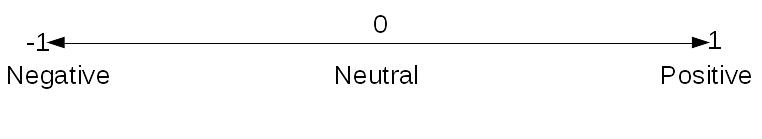
\includegraphics[scale=0.3]{sentiment_range.png}
\end{figure}
\begin{figure}
  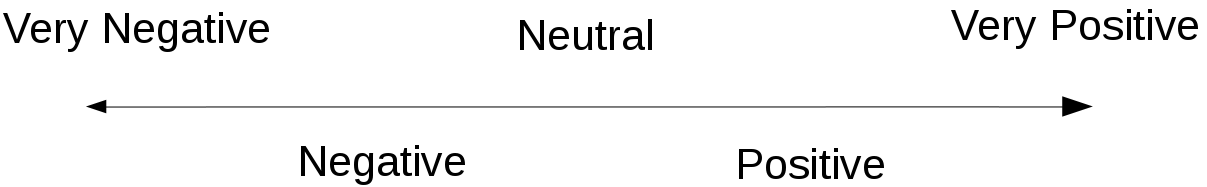
\includegraphics[scale=0.2]{long_sentiment_range.png}
\end{figure}
\end{block}
\end{frame}

\begin{frame}[fragile]{How is sentiment predicted}
  \begin{block}{Positive rotten tomato review}
    \begin{quote}
tim allen is \textcolor{blue}{great} in his role but never hogs the scenes from his fellow cast , as there are plenty of laughs and \textcolor{blue}{good} lines for everyone in this comedy. \citep{pang_2005}
    \end{quote}
  \end{block}
\end{frame}

\begin{frame}[fragile]{Sentiment within finance}
  \begin{block}{Finance Example}
    \begin{quote}
Falling \textcolor{red}{crude} prices, corrections make stocks \textcolor{blue}{attractive}\footnote{http://www.mydigitalfc.com/companies-and-markets/stock-market/falling-crude-prices-corrections-make-stocks-attractive}
    \end{quote}
  \end{block}
\end{frame}

\begin{frame}[fragile]{Sentiment within finance}
  \begin{block}{Finance Example}
    \begin{quote}
Falling crude prices, corrections make stocks \textcolor{blue}{attractive}\footnote{http://www.mydigitalfc.com/companies-and-markets/stock-market/falling-crude-prices-corrections-make-stocks-attractive}
    \end{quote}
  \end{block}
\end{frame}

\begin{frame}[fragile]{Sentiment within finance}
  \begin{block}{Finance Example}
    \begin{quote}
Falling crude prices, corrections make stocks \textcolor{blue}{attractive}\footnote{http://www.mydigitalfc.com/companies-and-markets/stock-market/falling-crude-prices-corrections-make-stocks-attractive}
    \end{quote}
  \end{block}

  \begin{block}{Shell Example}
    \begin{quote}
  Niger delta oil spill clean-up launched - but could take quarter of a century\footnote{\url{https://www.theguardian.com/global-development/2016/jun/02/niger-delta-oil-spill-clean-up-launched-ogoniland-communities-1bn}}
    \end{quote}
  \end{block}
\end{frame}

\begin{frame}[fragile]{Sentiment within finance}
  \begin{block}{Finance Example}
    \begin{quote}
Falling crude prices, corrections make stocks \textcolor{blue}{attractive}\footnote{http://www.mydigitalfc.com/companies-and-markets/stock-market/falling-crude-prices-corrections-make-stocks-attractive}
    \end{quote}
  \end{block}

  \begin{block}{Shell Example}
    \begin{quote}
  Niger delta oil \textcolor{red}{spill} clean-up launched - but could take quarter of a century\footnote{\url{https://www.theguardian.com/global-development/2016/jun/02/niger-delta-oil-spill-clean-up-launched-ogoniland-communities-1bn}}
    \end{quote}
  \end{block}
\end{frame}

\begin{frame}[fragile]{Finance specific word embeddings}
\center{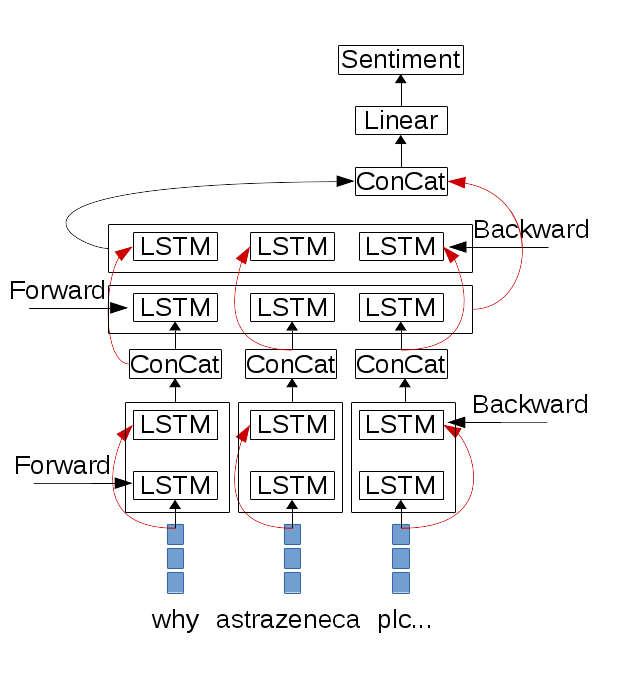
\includegraphics[scale=0.3]{lstm_diagram.png}}

\end{frame}

\begin{frame}[fragile]{What is the state of the art?}

\begin{table}[!h]
\centering
\scalebox{0.7}{
\begin{tabular}{|l|M|M|M|M|M|M|M|}
\hline
 &  \multicolumn{7}{c|}{Datasets}  \\
\hline
Methods & 1 & 2 & 3 & 4 & 5 & 6 & 7\\
 \hline
 \hline
 \textcite{mitchell_2013} &  &  & \cmark   & & & &\\
 \hline
 \textcite{kiritchenko_2014} &  &  &  & \cmark &  &  &\\
 \hline
 \textcite{dong_2014} & \cmark &  & & & & &\\
 \hline
 \textcite{vo_2015} & \cmark & \cmark & \cmark  & & & & \\
 \hline
 \textcite{zhang_2015} & &  & \cmark  & & & &\\
 \hline
 \textcite{zhang_2016} & \cmark & \cmark & \cmark  & & & & \\
 \hline
 \textcite{Tang_2016_tdlstm} & \cmark &   &  & \cmark & & &\\
 \hline
 \textcite{Tang_2016_mem} & & &   & \cmark & & &\\
 \hline
 \textcite{wang_2016} & &  & & \cmark & & &\\
 \hline
 \textcite{chen_2017} & \cmark &  &   & \cmark & \cmark & &\\
 \hline
 \textcite{liu_2017} & \cmark & \cmark & \cmark  &  & &  & \\
 \hline
 \textcite{wang_2017} & \cmark & &   &  &  & \cmark &\\
 \hline
 \textcite{Marrese_Taylor_2017} & &  & &   \cmark & &  & \cmark\\
 \hline
 \hline
\multicolumn{8}{|p{13.5cm}|}{1=\textcite{dong_2014}, 2=\textcite{wilson_2008}, 3=\textcite{mitchell_2013}, 4=\textcite{pontiki_2014}, 5=\textcite{chen_2017}, 6=\textcite{wang_2017}, 7=\textcite{Marrese_Taylor_2017}}\\
\hline
\end{tabular}
}
\caption{Methods and Datasets}
\label{table:methods_datasets}
\end{table}
\end{frame}


\begin{frame}[fragile]{Which implementation is correct?}
\begin{table}[!h]
\centering
\begin{tabular}{|l|c|c|}
\hline
Authors & Restaurant & Laptop \\
\hline
\textcolor{blue}{\textcite{Tang_2016_tdlstm}} & 75.63 & 68.13 \\
\hline
\textcolor{orange}{\textcite{chen_2017}} & 78.00 & 71.83 \\
\hline
\textcolor{red}{\textcite{tay_2017}} & 69.73 & 62.38 \\
\hline
\end{tabular}
\end{table}
\centering
\cbox{blue} Original\quad
\cbox{orange} Re-used the same code\quad
\cbox{red} Re-implemented

\end{frame}

\begin{frame}[fragile]{What we are doing}

\begin{table}[!h]
\centering
\scalebox{0.7}{
\begin{tabular}{|l|M|M|M|M|M|M|M|}
\hline
 &  \multicolumn{7}{c|}{Datasets}  \\
\hline
Methods & 1 & 2 & 3 & 4 & 5 & 6 & 7\\
 \hline
 \hline
 \textcite{mitchell_2013} &  &  & \cmark   & & & &\\
 \hline
 \textcite{kiritchenko_2014} &  &  &  & \cmark &  &  &\\
 \hline
 \textcite{dong_2014} & \cmark &  & & & & &\\
 \hline
 \alert{\textcite{vo_2015}} & \cmark & \cmark & \cmark  & & & & \\
 \hline
 \textcite{zhang_2015} & &  & \cmark  & & & &\\
 \hline
 \textcite{zhang_2016} & \cmark & \cmark & \cmark  & & & & \\
 \hline
 \alert{\textcite{Tang_2016_tdlstm}} & \cmark &   &  & \cmark & & &\\
 \hline
 \textcite{Tang_2016_mem} & & &   & \cmark & & &\\
 \hline
 \textcite{wang_2016} & &  & & \cmark & & &\\
 \hline
 \textcite{chen_2017} & \cmark &  &   & \cmark & \cmark & &\\
 \hline
 \textcite{liu_2017} & \cmark & \cmark & \cmark  &  & &  & \\
 \hline
 \alert{\textcite{wang_2017}} & \cmark & &   &  &  & \cmark &\\
 \hline
 \textcite{Marrese_Taylor_2017} & &  & &   \cmark & &  & \cmark\\
 \hline
 \hline
\multicolumn{8}{|p{13.5cm}|}{1=\textcite{dong_2014}, 2=\textcite{wilson_2008}, 3=\textcite{mitchell_2013}, 4=\textcite{pontiki_2014}, 5=\textcite{chen_2017}, 6=\textcite{wang_2017}, 7=\textcite{Marrese_Taylor_2017}}\\
\hline
\end{tabular}
}
\caption{Methods and Datasets}
\label{table:methods_datasets}
\end{table}
\end{frame}

\begin{frame}[fragile]{The future}

\begin{enumerate}
\item Transfer learning between related task
\item Transfer learning between languages
\end{enumerate}

\end{frame}

%
% Ignore
%




\begin{frame}[plain]
\begin{center}
\begin{center}
\huge Questions?
\end{center}
\begin{center}
\begin{columns}[T,onlytextwidth]
\column{0.1\textwidth}
\column{0.4\textwidth}
\centering
\normalsize a.moore@lancaster.ac.uk
\column{0.4\textwidth}
\centering
\normalsize @apmoore94
\column{0.1\textwidth}
\end{columns}
\end{center}
\end{center}

\begin{center}
\begin{center}
\small Presentation can be found here \footnote{\url{https://github.com/apmoore1/presentations/blob/master/SCC\%20PhD\%20Conference/slides.pdf}}
\end{center}
\end{center}

\end{frame}


\appendix
\begin{frame}[noframenumbering,plain,allowframebreaks]{References}
  \printbibliography[heading=none]
\end{frame}

\end{document}

